The first broad classification of link prediction methods explored in this thesis are the knowledge graph embedding methods (KGE).
Since graph neural networks generate node embeddings as well, the terminology is somewhat ambiguous.
The following few paragraphs will attempt to distinguish the class of methods detailed in this chapter.

KGE methods attempt to position each node in a vector space (figure~\ref{fig:vec-space-vis}).
In a well-trained model, nodes from the same neighborhood will be placed near each other within the vector space.
Moreover, these positions are strictly unique, i.e., \ two distinct nodes cannot occupy the same place.
From this, it naturally follows that KGE methods are strictly transductive and cannot be generalized.

Fortunately, a transductive setting is not necessarily limiting for the purposes of this thesis.
as all the link-predictions tasks are limited
to the domain of places mentioned in Kitāb Mu'jam al-Buldān.

KGE methods are generally more efficient and easily more scalable than their GNN counterparts.


\begin{figure}[h] % [h] attempts to place figure here, other options like [t]op, [b]ottom
    \centering % Centers the figure horizontally
    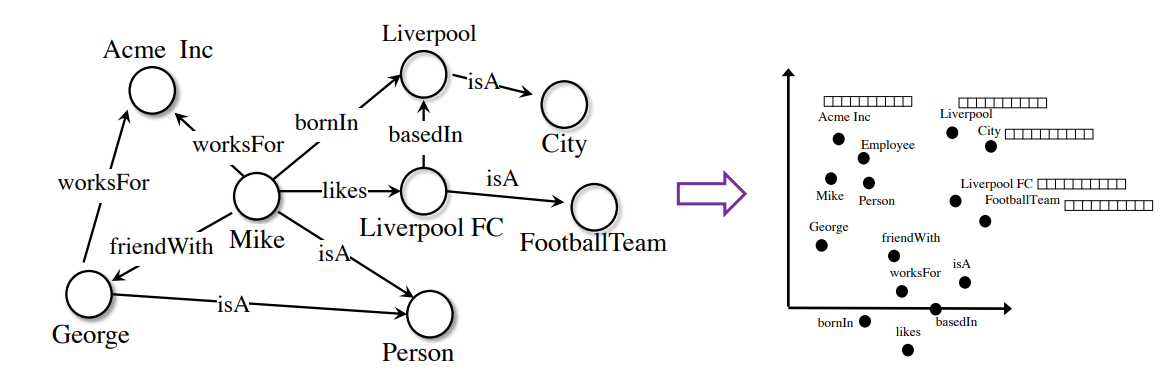
\includegraphics[width=1\linewidth]{figures/vector-space} % Include the image with desired width
    \caption{Visualization of Vector Space Embedding~\cite{KGETutorial}} % Add a caption
    \label{fig:vec-space-vis} % Assign a label for referencing the figure in text
\end{figure}.